\documentclass[border=2mm]{standalone}

\usepackage{fontspec}
\usepackage{unicode-math}
\usepackage{amsmath}

\usepackage{pgfplots}
\pgfplotsset{compat=1.18}
\usetikzlibrary{arrows.meta, 
  calc, 
  positioning, 
  decorations.pathreplacing, 
  calligraphy}
\usetikzlibrary{patterns}

\usepackage{xcolor}
\definecolor{den-1}{HTML}{111111}   % Đen #111111
\definecolor{den-2}{HTML}{222222}   % Đen #222222
\definecolor{den-3}{HTML}{333333}   % Đen #333333
\definecolor{den-4}{HTML}{444444}   % Đen #444444
\definecolor{den-5}{HTML}{555555}   % Đen #555555
\definecolor{den-6}{HTML}{666666}   % Đen #666666


\begin{document}

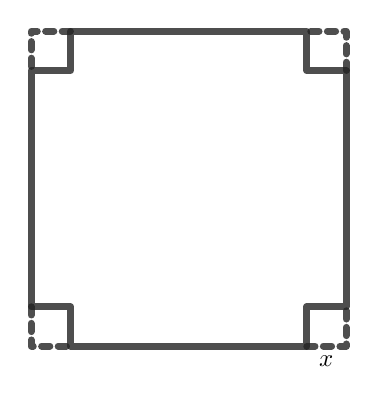
\begin{tikzpicture}[scale=1, line cap=round, line join=round]

  \draw [line width=2.5pt, color=den-2, opacity=.8] 
    (.5,0) -- (3.5,0) -- (3.5,.5) -- (4,.5) -- (4,3.5) -- (3.5,3.5) -- (3.5,4) -- (.5,4) -- (.5,3.5) -- (0,3.5) -- (0,.5) -- (.5,.5) -- cycle;

  % \draw [line width=2.5pt, color=den-2, opacity=.8]
  %   (.5,.5) -- (3.5,.5) -- (3.5,3.5) -- (.5,3.5) -- cycle;
      
  
  \draw [dashed, line width=2.5pt, color=den-2, opacity=.8] 
    (0,.5) -- (0,0) -- (.5,0);

  \draw [dashed, line width=2.5pt, color=den-2, opacity=.8] 
    (3.5,0) -- (4,0) -- (4,.5);

  \draw [dashed, line width=2.5pt, color=den-2, opacity=.8] 
    (4,3.5) -- (4,4) -- (3.5,4);

  \draw [dashed, line width=2.5pt, color=den-2, opacity=.8] 
    (.5,4) -- (0,4) -- (0,3.5);

  % Nhãn
  \node at (3.75,0) [below] {\small $x$};
  

  % Mũi tên cong và ghi chú thể tích

  % \draw [->, thick, color=den-4, rounded corners=10pt] 
  %   (2,3.5) to[bend left=30] (3.5,2.5);

  % \node at (2,3.5) [above] {\small $500\,\text{cm}^3$};

\end{tikzpicture}


\end{document}
